\documentclass{article}

\usepackage{amssymb}
\usepackage{amsthm}
\usepackage[UKenglish]{babel}
\usepackage{enumitem}
\usepackage{fancyhdr}
\usepackage[margin=1in]{geometry}
\usepackage{graphicx}
\usepackage[utf8]{inputenc}
\usepackage{listings}
\usepackage{mathtools}
\usepackage{tikz-cd}
\usepackage{csquotes}

\newcommand{\F}{\mathbb{F}}
\newcommand{\N}{\mathbb{N}}
\newcommand{\Z}{\mathbb{Z}}
\newcommand{\Q}{\mathbb{Q}}
\newcommand{\R}{\mathbb{R}}
\newcommand{\C}{\mathbb{C}}
\newcommand{\A}{\mathbb{A}}
\renewcommand{\P}{\mathbb{P}}

\newcommand{\val}[1]{\left. #1 \right\rvert}
\newcommand{\rb}[1]{\left( #1 \right)}
\renewcommand{\sb}[1]{\left[ #1 \right]}
\newcommand{\cb}[1]{\left\{ #1 \right\}}
\newcommand{\ab}[1]{\left\langle #1 \right\rangle}
\newcommand{\abs}[1]{\left\lvert #1 \right\rvert}
\newcommand{\two}[2]{\begin{pmatrix} #1 \\ #2 \end{pmatrix}}
\newcommand{\three}[3]{\begin{pmatrix} #1 & #2 & #3 \end{pmatrix}}

\theoremstyle{definition}\newtheorem{definition}{Definition}[section]
\theoremstyle{definition}\newtheorem{remark}[definition]{Remark}
\theoremstyle{definition}\newtheorem*{example}{Example}
\theoremstyle{definition}\newtheorem*{note}{Note}
\newtheorem{proposition}[definition]{Proposition}
\newtheorem{lemma}[definition]{Lemma}
\newtheorem{theorem}[definition]{Theorem}
\newtheorem{corollary}[definition]{Corollary}
\newtheorem{algorithm}[definition]{Algorithm}

\pagestyle{fancy}
\lhead{M4P32 Number Theory: Elliptic Curves}
\rhead{Autumn 2018}

\title{M4P32 Number Theory: Elliptic Curves}
\author{Lectured by Prof Toby Gee \\ Typeset by David Kurniadi Angdinata}
\date{Autumn 2018}

\setcounter{section}{-1}

\begin{document}

\maketitle

\vfill

\tableofcontents

\pagebreak

\marginpar{Lecture 1 \\ Thursday \\ 04/10/18}

\section{Introduction}

\subsection{Outline}

\begin{enumerate}
\item Introduction
\item Conics
\begin{enumerate}
\item The $ p $-adic numbers
\item Basic algebraic geometry
\item Plane curves
\item The Hasse principle
\end{enumerate}
\item Cubics
\begin{enumerate}
\item Definitions
\item Elliptic curves over $ \Q_p $
\item Elliptic curves over $ \Q $
\item The Mordell-Weil theorem
\end{enumerate}
\end{enumerate}

The theme of the course will be studying polynomial equations over $ \Z $ or $ \Q $.

\begin{example}
For $ x^7 + y^7 + z^7 = 1 $, what are the solutions with $ x, y, z \in \Q $? Answer is hard. However $ x^2 - 1 = 0 $ is easy. In fact any equation in one variable is easy to solve over $ \Q $. For example, $ 3x^5 - 9x^3 + x^2 + 148 / 81 = 0 $ iff $ 243x^5 - 729x^3 + 81x^2 + 148 = 0 $. Letting $ x = r / s $ for $ \rb{r, s} = 1 $ and $ s \ge 1 $, such as $ r = -2 $ and $ s = 5 $ in $ -2 / 5 $, gives $ 243r^5 - 729r^3s^2 + 81r^2s^3 + 148s^5 = 0 $. So $ r^2 \mid 148s^5 $, but $ \rb{r, s} = 1 $, so $ r^2 \mid 148 $. Similarly $ s^2 \mid 243 $. Now check the finitely many possibilities to get $ x = 2 / 3 $ as the only solution in $ \Q $.
\end{example}

If $ k $ is a field, such as $ \Q $, $ \R $, $ \C $, $ \F_p $, $ \Q_p $, we write $ k\sb{x_1, \dots, x_n} $ for the polynomial ring in $ n $ variables $ x_1, \dots, x_n $. A \textbf{monomial} is an expression $ x_1^{\alpha_1}, \dots, x_n^{\alpha_n} $ for $ a_i \in \Z_{> 0} $. The \textbf{degree} of $ x_1^{\alpha_1}, \dots, x_n^{\alpha_n} $ is $ a_1 + \dots + a_n $. An element of $ k\sb{x_1, \dots, x_n} $ is just a finite sum of multiples of monomials with coefficients in $ k $. Its degree is the largest degree of any monomial occurring in it. For example, $ 5x_{10}^3 + x_2x_3^{10} - \rb{2 / 3}x_1^7 $ has degree $ 11 $. Typically we will be looking at the case of two variables $ x_1, x_2 $, which we will usually call $ x, y $.

\begin{theorem}[Falting's theorem]
The general equation in two variables of degree greater than four over $ \Q $ is known to only have finitely many solutions in $ \Q $.
\end{theorem}

\begin{example}
$ x^4 + y^4 = 17 $ only has $ \rb{\pm 1, \pm 2} $ and $ \rb{\pm 2, \pm 1} $ as solutions, which is proved only in 2001. $ \rb{x^{100} + 5y^{100} - 7}\rb{x - y} = 0 $ is not a general equation and has infinitely many solutions.
\end{example}

\begin{example}
$ x^2 + y^2 = -1 $ has no solutions in $ \Q $. $ x^2 + y^2 = 0 $ has finitely many solutions in $ \Q $ $ \rb{x = y = 0} $. $ x^2 + y^2 = 1 $ has infinitely many solutions in $ \Q $. Let $ x = a / c $ and $ y = b / c $ for $ a, b, c \in \Z $ gives Pythagorean triples $ a^2 + b^2 = c^2 $, such as $ 3^2 + 4^2 = 5^2 $, $ 5^2 + 12^2 = 13^2 $, etc.
\end{example}

\begin{example}
$ x^2 + y^2 = 3 $ has solutions in $ \R $ but no solutions in $ \Q $. Equivalently, $ a^2 + b^2 = 3c^2 $ has no solutions with $ a, b, c \in \Z $ except $ a = b = c = 0 $. Suppose we have a solution. Then $ a^2 + b^2 \equiv 0 \mod 3 $. A fact is that if $ n \in \Z $, then $ n^2 \equiv 0 \mod 3 $ if $ 3 \mid n $, or $ n^2 \equiv 1 \mod 3 $ if $ 3 \nmid n $. So $ a \equiv b \equiv 0 \mod 3 $, or $ 3 \mid a, b $. Write $ a = 2A $ and $ b = 3B $. Then $ \rb{3A}^2 + \rb{3B}^2 = 3c^2 $ iff $ 9\rb{A^2 + B^2} = 3c^2 $, iff $ 3\rb{A^2 + B^2} = c^2 $. So $ 3 \mid c^2 $ and $ 3 \mid c $. Write $ c = 3C $. Then $ 3\rb{A^2 + B^2} = \rb{3C}^2 $ iff $ 3\rb{A^2 + B^2} = 9C^2 $, iff $ A^2 + B^2 = 3C^2 $. Thus $ a = b = c = 0 $.
\end{example}

$ x^2 + y^2 = -1 $ has an obstruction in $ \R $. $ x^2 + y^2 = 3 $ has an obstruction in $ \Q_3 $. Hasse principle will tell us that for general equations of degree two in $ x, y $, there are either infinitely many solutions in $ \Q $ or no solutions, and furthermore either no solutions in $ \R $ or no solutions in $ \Q_p $ for some prime $ p $.

\marginpar{Lecture 2 \\ Friday \\ 05/10/18}

We study plane conics and plane cubics. Plane refers to 2 variables $ x, y $. Conic refers to degree two while cubic refers to degree three.

\begin{example}
$ x^2 + 2y^2 = 6 $ has a rational solution $ \rb{2, 1} $. Drawing lines at $ \rb{2, 1} $ with rational slope $ y - 1 = m\rb{x - 2} $ will get all rational solutions by intersecting with $ x^2 + 2y^2 = 6 $. Then $ x^2 + 2\rb{m\rb{x - 2} + 1}^2 = 6 $ gives $ \rb{2m^2 + 1}x^2 + 4m\rb{1 - 2m}x + 2\rb{2m^2 - 1}^2 = 0 $. The sum of the roots of this equation is $ 4m\rb{2m - 1} / \rb{2m^2 + 1} $. Since $ x = 2 $ is a root, the other root is
$$ x_0 = \dfrac{4m\rb{2m - 1}}{2m^2 + 1} - 2 = \dfrac{4m^2 - 4m - 2}{2m^2 + 1}, \qquad y_0 = m\rb{x_0 - 2} + 1 = m\rb{\dfrac{-4m - 4}{2m^2 + 1}} + 1 = \dfrac{-2m^2 - 4m + 1}{2m^2 + 1}. $$
If $ m \in \Q $, $ \rb{x_0, y_0} \in \Q^2 $ and conversely, which is easy. For example, $ m = 1 $ gives $ \rb{x_0, y_0} = \rb{-2 / 3, -5 / 3} $ and $ m \to \infty $ gives $ \rb{x_0, y_0} \to \rb{2, -1} $. (TODO Exercise: for $ x^2 + y^2 = 1 $, $ x^2 + y^2 = 0 $, $ xy = 0 $, $ x^2 - y^2 = 0 $)
\end{example}

\subsection{References}

\begin{enumerate}
\item J W S Cassels, Lectures on elliptic curves, 1991
\item J H Silverman, The arithmetic of elliptic curves, 1986
\item J H Silverman and J Tate, 1992
\end{enumerate}

\pagebreak

\section{The $ p $-adic numbers}

\begin{definition}
A \textbf{norm} on a field $ k $ is a function $ \abs{\cdot} : k \to \R $ such that:
\begin{enumerate}
\item $ \abs{x} \ge 0 $ with equality iff $ x = 0 $,
\item $ \abs{xy} = \abs{x}\abs{y} $, and
\item $ \abs{x + y} \le \abs{x} + \abs{y} $.
\end{enumerate}
\end{definition}

\begin{note}
$ \abs{1} = \abs{-1} = 1 $ and $ \abs{-x} = \abs{-1}\abs{x} = \abs{x} $.
\end{note}

\begin{example}
Let $ k = \Q $ or $ \R $ and $ \abs{x} $ is the absolute value of $ x $, that is $ \abs{x} = x $ if $ x \ge 0 $ and $ \abs{x} = -x $ if $ x < 0 $.
\end{example}

\begin{example}
Discrete norm $ \abs{x} = 0 $ if $ x = 0 $ and $ \abs{x} = 1 $ if $ x \ne 0 $.
\end{example}

\begin{remark}
Any norm on $ k $ defines a metric by $ d\rb{x, y} = \abs{x - y} $. In particular, a norm determines a topology.
\end{remark}

\begin{example}
The discrete norm determines the discrete topology.
\end{example}

\begin{definition}
Let $ p $ be a prime number. Let $ a / b \in \Q $ with $ \rb{a, b} = 1 $. Let $ p^n $ be the biggest power of $ p $ dividing $ a / b $, so $ a / b = p^n \rb{c / d} $ with $ \rb{c, p} = \rb{d, p} = 1 $. Then the \textbf{$ p $-adic norm} is $ \abs{a / b}_p = p^{-n} $.
\end{definition}

\begin{example}
$ \abs{1 / 6}_5 = 1 $, $ \abs{1 / 6}_3 = 3 $. $ p^n \to 0 $ into the $ p $-adic topology as $ n \to \infty $.
\end{example}

\begin{lemma}
$ \abs{\cdot}_p $ is a norm on $ \Q $.
\end{lemma}

\begin{proof}
\hfill
\begin{enumerate}
\item Trivial.
\item Unique factorisation.
\item Prove $ 3' : \abs{x + y}_p \le \max\rb{\abs{x}_p, \abs{y}_p} $. Without loss of generality, $ x, y, x + y \ne 0 $. Multiplying $ x, y $ by any power of $ p $ does not affect the truth of $ 3' $, so without loss of generality $ x, y \in \Z $. Then we have to show that $ p^r \mid x $ and $ p^r \mid x + y $, which is obvious.
\end{enumerate}
\end{proof}

$ 3' $ is the \textbf{ultrametric inequality}.

\begin{definition}
If $ \abs{\cdot} $ satisfies $ 3' $, we say that $ \abs{\cdot} $ is \textbf{nonarchimedean}. Otherwise $ \abs{\cdot}_p $ is \textbf{archimedean}.
\end{definition}

Say that two norms $ \abs{\cdot}_1 $, $ \abs{\cdot}_2 $ on a field $ k $ are equivalent if $ \abs{\cdot}_1 = \abs{\cdot}_2^\alpha $ for some $ \alpha > 0 $. If two norms are equivalent, they define the same topology. \textbf{Ostrowski's theorem} states that up to equivalence, the only norms on $ \Q $ are the usual archimedean norm, the discrete norm, and the $ p $-adic norms.

\marginpar{Lecture 3 \\ Tuesday \\ 09/10/18}

\begin{lemma}
\label{lem:1.6}
If $ \abs{\cdot} $ is nonarchimedean and $ \abs{x} \ne \abs{y} $, then $ \abs{x + y} = \max\rb{\abs{x}, \abs{y}} $.
\end{lemma}

\begin{proof}
Without loss of generality, $ \abs{x} > \abs{y} $. Write $ x = \rb{x + y} + \rb{-y} $, so $ \abs{x} \le \max\rb{\abs{x + y}, \abs{-y}} $. So equality holds in all inequalities, so $ \abs{x} = \abs{x + y} $.
\end{proof}

\begin{example}
Think about $ D\rb{a, r} = \cb{x \mid \abs{x - a} < r} $ and $ D\rb{b, r} = \cb{x \mid \abs{x - b} < r} $. What are the possibilities for $ D\rb{a, r} \cap D\rb{b, r} $?
\end{example}

(TODO Exercise: directly prove Lemma \ref{lem:1.6} from the definition) Let $ k $ be a field, let $ \abs{\cdot} $ be any norm on $ k $. $ d\rb{x, y} = \abs{x - y} $ is a metric, so $ k $ is a metric space with metric $ d $. We have the usual definitions for sequences $ \rb{x_n} $. Say that $ x_n $ \textbf{converges} to $ x $ if for all $ \epsilon > 0 $, there exists $ N $ such that $ n \ge N $ gives $ \abs{x_n - x} < \epsilon $. Say that $ \rb{x_n} $ is \textbf{Cauchy} if $ \epsilon > 0 $, there exists $ N $ such that $ m, n \ge N $ gives $ \abs{x_n - x_m} < \epsilon $. Say that $ \rb{x_n} $ is \textbf{convergent} if $ x_n $ converges to $ x $ for some $ x \in k $. Write $ x_n \to x $. If $ \rb{x_n} $ is convergent, then $ \rb{x_n} $ is Cauchy. Say that $ k $ is \textbf{complete} with respect to $ \abs{\cdot} $ if all Cauchy sequences converge.

\begin{example}
Let $ k = \Q $ with the usual archimedean norm $ \abs{\cdot} $. $ 1, 1.4, 1.41, 1.414, \dots \to \sqrt{2} \notin \Q $.
\end{example}

\begin{example}
Let $ k = \Q $ with $ \abs{\cdot}_2 $. $ 3, 33, 333, 3333, \dots $ is a Cauchy sequence. In fact, if $ m > n $, $ \abs{x_m - x_n}_2 = 2^{-n} $. So if $ m, n \ge N $, $ \abs{x_m - x_n} \le 2^{-N} $. $ x_n = \rb{10^n - 1} / 3 $ so $ x_n + 1 / 3 = 10^n / 3 = 2^n\rb{5^n / 3} $. $ \abs{x_n + 1 / 3}_2 = 2^{-n} $, so $ x_n + 1 / 3 \to 0 $.
\end{example}

\begin{example}
Let $ k = \Q $ with $ \abs{\cdot}_5 $. $ \abs{5^{2^n}}_5 = 5^{-2^n} \to 0 $ as $ n \to \infty $.
\end{example}

\begin{example}
Let $ k = \Q $ with $ \abs{\cdot}_2 $. $ \rb{5^{2^n}} $ is $ 5, 25, 625, \dots \to 1 $. Want to show that $ 5^{2^n} - 1 \to 0 $, so that bigger and bigger powers of two divide $ 5^{2^n} - 1 $. Use the lemma that $ t \equiv 1 \mod 2^k $ gives $ t^2 \equiv 1 \mod 2^{k + 1} $.
\end{example}

\begin{example}
Let $ k = \Q $ with $ \abs{\cdot}_7 $. $ 5^{2^n} $ is not Cauchy. In fact $ \mod 7 $ it looks like $ 5, 4, 2, 4, 2, \dots $, so $ \abs{x_n - x_{n + 1}}_7 = 1 $.
\end{example}

\begin{example}
An example of a Cauchy sequence in $ \Q $ for some $ \abs{\cdot}_p $ which does not converge. Want to find a Cauchy sequence $ \rb{x_n} $ with $ x_n^2 \to 7 $, so write down a sequence $ \rb{x_n} $ such that $ \abs{x_n^2 - 7}_3 \to 0 $. If $ x_1 = 1 $, then $ x_1^2 \equiv 7 \mod 3 $. If $ x_2 = 4 $, then $ x_2^2 \equiv 7 \mod 9 $. Find some $ n \in \N $ such that $ x_3 = 4 + 9n $ and $ x_3^2 \equiv 7 \mod 27 $. $ x_3^2 = \rb{4 + 9n^2} = 16 + 8\rb{9n} + \rb{9n}^2 \equiv 16 + 8\rb{9n} \mod 27 $. So want $ 9 + 8\rb{9n} \equiv 0 \mod 27 $, so $ 1 + 8n \equiv 0 \mod 3 $, such as $ n = 1 $. So $ x_3 = 13 $. Similar $ x_4 = 13 + 27n $ and find some $ n \in \N $.
\end{example}

\begin{example}
Show that for all primes $ p $ there is a Cauchy sequence $ \rb{x_n} $ in $ \Q $ for $ \abs{\cdot}_p $ with the property that $ x_n^2 \to t $ for some integer $ t $ which is not a perfect square, such as $ t = 1 - p $ if $ p > 2 $ and $ t = -7 $ if $ p = 2 $. (TODO Exercise)
\end{example}

There is a general notion of completing a field with respect to a norm. The result is a field $ K $ containing $ k $, for which all Cauchy sequences in $ k $ converge, and such that $ K $ is minimal with this property.

\begin{example}
Let $ k = \Q $ with the archimedean norm $ \abs{\cdot} $, then $ K = \R $.
\end{example}

\marginpar{Lecture 4 \\ Thursday \\ 11/10/18}

Let $ k $ be a field and $ \abs{\cdot} $ be a norm on $ k $. Let $ R $ be the ring of Cauchy sequences in $ k $, so elements of $ R $ are $ \rb{x_n} $ for $ x_n \in k $, where $ \rb{x_n} + \rb{y_n} = \rb{x_n + y_n} $ and $ \rb{x_n}\rb{y_n} = \rb{x_ny_n} $.

Let $ I = \cb{\rb{x_n} \in R \mid x_n \to 0 \text{ as } n \to \infty} $. Claim that $ I $ is an ideal in $ R $. $ \rb{x_n}, \rb{y_n} \in I $ then $ \rb{x_n + y_n} \in I $ because $ x_n \to 0 $ and $ y_n \to 0 $ gives $ x_n + y_n \to 0 $. If $ \rb{x_n} \in R $, $ \rb{y_n} \in I $ then $ \rb{x_n} $ is bounded, so $ x_ny_n \to 0 $.

Define the completion of $ k $ to be $ \widehat{k} = R / I $. Claim that $ \widehat{k} $ is a field, so $ I $ is a maximal ideal of $ R $. Need to show that if $ \rb{x_n} \in R $ with $ x_n \not\to 0 $, then there exists $ \rb{y_n} \in R $ such that $ \rb{x_ny_n} \in 1 + I $. $ x_n \not\to 0 $ gives $ \epsilon, N $ such that $ n \ge N $ gives $ \abs{x_n} \ge \epsilon > 0 $. Set $ y_n = 0 $ if $ n < N $ and $ y_n = 1 / x_n $ if $ n \ge N $. Show that $ \rb{y_n} \in R $. (TODO Exercise) Then $ \rb{x_ny_n} = 0 $ if $ n < N $ and $ \rb{x_ny_n} = 1 $ if $ n \ge N $, so $ x_ny_n \to 1 $ as $ n \to \infty $, as required.

$ k $ is a subfield of $ \widehat{k} $ by $ x \mapsto \rb{x} $. Check that $ \widehat{k} $ has a natural norm extending $ \abs{\cdot} $ on $ k $, and $ \widehat{k} $ is complete with respect to this norm, so $ \abs{\rb{x_n}} = \lim_{n \to \infty} \abs{x_n} $. (TODO Exercise)

Prove that if $ \abs{\cdot} $ on $ k $ is a nonarchimedean norm, then so is the induced norm on $ \widehat{k} $. (TODO Exercise) Furthermore, the sequence $ \abs{x_n} $ is eventually constant for any Cauchy sequence $ \abs{x_n} \in R \setminus I $. (TODO Exercise)

\begin{note}
For $ \abs{\cdot}_p $ on $ \Q $ this means that $ \abs{\cdot} $ is taking values in $ p^{\Z} $.
\end{note}

\begin{definition}
The \textbf{$ p $-adic numbers} $ \Q_p $ is the completion of $ \Q $ with respect to the $ p $-adic norm. The \textbf{$ p $-adic integers} $ \Z_p $ is the closed unit disc in $ \Q_p $, so $ \Z_p = \cb{x \in \Q_p \mid \abs{x}_p = 1} $.
\end{definition}

Prove that $ \Z_p $ is a subring of $ \Q_p $. Use that $ \abs{\cdot}_p $ is nonarchimedean. (TODO Exercise) Also $ \Q \cap \Z_p = \cb{r / s \mid \rb{r, s} = 1, \ p \nmid s} $. In particular $ \Z \subset \Z_p $. (TODO Exercise)

Prove that $ \Q $ is dense in $ \Q_p $. Indeed $ k $ is dense in $ \widehat{k} $. (TODO Exercise) A less obvious fact is that $ \Z $ is dense in $ \Z_p $.

\begin{definition}
Let $ k $ be a field with a norm $ \abs{\cdot} $, and $ \rb{x_n} $ be any sequence. Then $ \sum_{n = 1}^\infty = \lim_{N \to \infty} \sum_{n = 1}^N x_n $, if this limit exists.
\end{definition}

\begin{lemma}
\label{lem:1.10}
If $ k $ is nonarchimedean and $ x_1, \dots, x_r $ satisfy $ \abs{x_i} \le R $ for some $ R $, then $ \abs{\sum_{n = 1}^r x_i} \le R $.
\end{lemma}

\begin{proof}
Induction with ultrametric inequality.
\end{proof}

\begin{corollary}
\label{cor:1.11}
If $ k $ is nonarchimedean then $ \rb{x_n} $ is Cauchy iff $ x_n - x_{n + 1} \to 0 $ as $ n \to \infty $.
\end{corollary}

\begin{proof}
Forward direction is obvious. Conversely, $ m > n $ gives $ x_m - x_n = \rb{x_m - x_{m - 1}} + \dots + \rb{x_{n + 1} - x_n} $. If $ \abs{x_{i + 1} - x_i} \le \epsilon $ for all $ i \ge N $ then $ \abs{x_m - x_n} \le \epsilon $ for all $ m, n \ge N $ by Lemma \ref{lem:1.10}.
\end{proof}

\begin{lemma}
\label{lem:1.12}
If $ k $ is complete and nonarchimedean then $ \sum_{n = 1}^\infty x_n $ converges iff $ x_n \to 0 $ as $ n \to \infty $. If $ \abs{x_n}^{n - 1} \le R $ for all $ n $ and $ x_n \to 0 $ then $ \abs{\sum_{n = 1}^\infty x_n} \le R $.
\end{lemma}

\begin{proof}
Apply Lemma \ref{lem:1.10} and Corollary \ref{cor:1.11} to the sequence $ \rb{\sum_{i = 1}^n x_i} $.
\end{proof}

\begin{lemma}
\label{lem:1.13}
If $ a_n \in \Z $ for all $ n \ge 0 $, then $ \sum_{n = 0}^\infty a_np^n $ converges in $ \Q_p $. If $ a_n = 0 $ for $ n < T $ and $ p \nmid a_T $ then $ \abs{\sum_{n = 0}^\infty a_np^n} = p^{-T} $.
\end{lemma}

\begin{proof}
$ \abs{a_np^n}_p \le \abs{p^n}_p = p^{-n} \to 0 $ as $ n \to \infty $, so $ \sum_{n = o}^N a_np^n $ converges by Lemma \ref{lem:1.12}. If $ N \ge T $ then $ \abs{\sum_{n = o}^N a_np^n} = p^{-T} $. (TODO Exercise: use lemma \ref{lem:1.6})
\end{proof}

\begin{proposition}
\label{prop:1.14}
\hfill
\begin{enumerate}
\item If $ a_n \in \cb{0, \dots p - 1} $, then $ \sum_{n = 0}^\infty a_np^n \in \Z_p $. Further more if $ a_n, b_n \in \cb{0, \dots, p - 1} $ and $ \sum_{n = 0}^\infty a_np^n = \sum_{n = 0}^\infty b_np^n $ then $ a_n = b_n $ for all $ n $.
\item If $ x \in \Z_p $ then there is a unique sequence $ \rb{a_n} $ as in 1 with $ x = \sum_{n = 0}^\infty a_np^n $.
\end{enumerate}
\end{proposition}

\begin{proof}
\hfill
\begin{enumerate}
\item Convergence is Lemma \ref{lem:1.13}. If $ \rb{a_n} \ne \rb{b_n} $ let $ T $ be minimal such that $ a_T \ne b_T $. Then
$$ \abs{\sum_{n = 0}^\infty a_np^n - \sum_{n = 0}^\infty a_np^n} = \abs{\sum_{n = 0}^\infty \rb{a_n - b_n}p^n} = p^{-T} $$
by Lemma \ref{lem:1.13}, so $ \sum_{n = 0}^\infty a_np^n \ne \sum_{n = 0}^\infty a_np^n $.
\item Let $ x \in \Z_p $. Since $ \Q $ is dense in $ \Q_p $ by construction, there exists $ r / s \in \Q $, $ \rb{r, s} = 1 $ with $ \abs{x - r / s}_p < 1 $. Since $ \abs{x}_p \le 1 $, $ \abs{r / s}_p \le 1 $, so $ p \nmid s $. So there exists $ \gamma \in \Z $ with $ \abs{\gamma - r / s}_p < 1 $, so $ s\gamma \equiv r \mod p $. Then $ \abs{\gamma - x}_p < 1 $. Now choose $ a_0 \in \cb{0, \dots, p - 1} $ with $ \gamma \equiv a_0 \mod p $. Then $ \abs{a_0 - x}_p < 1 $. So $ \abs{\rb{a_0 - x} / p}_p \le 1 $, and repeating the process, there exists $ a_1 \in \cb{0, \dots, p - 1} $ with $ \abs{\rb{a_0 - x} / p - a_1}_p < 1 $, and so on. $ \abs{x - a_0 - a_1p}_p \le 1 / p^2 $, etc.
\end{enumerate}
\end{proof}

\marginpar{Lecture 5 \\ Friday \\ 12/10/18}

\begin{corollary}
Every element of $ \Q_p $ has a unique expression as $ a = \sum_{n \ge -T} a_np^n $ for $ a_n \in \cb{0, \dots, p - 1} $, $ a_{-T} \ne 0 $, and $ \abs{a}_p = p^T $.
\end{corollary}

\begin{proof}
Given $ a \in \Q_p $, let $ T $ be such that $ \abs{a}_p = p^T $. Apply Proposition \ref{prop:1.14} to $ p^Ta $.
\end{proof}

\begin{corollary}
$ \Z $ is dense in $ \Z_p $.
\end{corollary}

\begin{proof}
If $ a \in \Z_p $, write $ a = \sum_{n = 0}^\infty a_np^n $. Then $ \sum_{n = 0}^N a_np^n $ is a sequence in $ \Z $ which converges to $ a $.
\end{proof}

For each $ n \ge 1 $ there is a ring homomorphism $ \Z_p \to \Z / p^n\Z $ that sends $ \sum_{i = 0}^\infty a_ip^i \mapsto \sum_{i = 0}^n a_ip^i $. The kernel of this map is $ p^n\Z_p $, so $ \Z_p / p^n\Z_p \cong \Z / p^n\Z $.

\begin{note}
In fact, $ \Z_p \cong \lim_{\leftarrow n} \Z / p^n\Z $.
\end{note}

$ p\Z_p $ is a maximal ideal of $ \Z_p $ because $ \Z_p / p\Z_p = \Z / p\Z $ is a field. If $ a \in \Z_p $, $ a \notin p\Z_p $, then $ a \in \Z_p^* $. Write $ a = a_0 + pa_1 + \dots $ for $ a_0 \in \cb{1, \dots, p - 1} $.

\begin{example}
$ a = a_0 + pA $. Show that $ a $ has an inverse using the formula for the sum of a geometric progression. (TODO Exercise) For example $ \rb{1 - p}^{-1} = 1 + p + \dots $.
\end{example}

Alternatively, $ a \in \Z_p $ is in $ p\Z_p $ iff $ \abs{a}_p < 1 $. So if $ a \in \Z_p \setminus p\Z_p $, then $ \abs{a}_p = 1 $. Then $ \abs{1 / a}_p = 1 / \abs{a}_p = 1 $, so $ 1 / a \in \Z_p $. $ 1 / a $ exists because $ \Q_p $ is a field. So $ p\Z_p $ is the unique maximal ideal of $ \Z_p $, so $ \Z_p $ is a local ring. $ \Z_p^* = \Z_p \setminus p\Z_p $ is the group of units. Terminology: $ a \in \Q_p $ is a \textbf{unit} iff $ a \in \Z_p^* $, so iff $ \abs{a}_p = 1 $.

\begin{lemma}
$ a \in \Z_p^* $ iff $ \abs{a}_p = 1 $.
\end{lemma}

\begin{proof}
(TODO above)
\end{proof}

\begin{corollary}
Every element of $ \Q_p^* = \Q_p \setminus \cb{0} $ is uniquely of the form $ p^nu $ for $ n \in \Z $ and $ u \in \Z_p^* $.
\end{corollary}

\begin{proof}
Set $ \abs{a}_p = p^{-n} $, then $ \abs{p^{-n}a}_p = 1 $, so $ u = p^{-n}a $, so $ a = up^n $.
\end{proof}

Aim is to solve the equation $ x^2 - 7 = 0 $ in $ \Z_3 $ starting with a solution to $ x^2 \equiv 7 \mod 3 $. We did this by solving $ x^2 \equiv 7 \mod 3^n $ for $ n = 1, 2, \dots $. Write $ f\rb{x} = x^2 - 7 $. Then $ \abs{f\rb{1}}_3 = 1 / 3 $, $ \abs{f\rb{4}}_3 = 1 / 9 $, $ \abs{f\rb{13}}_3 = 1 / 27 $, etc. So starting with $ x_0 = 1 $, we construct a sequence $ \rb{x_n} $ with $ \abs{x_{n + 1} - x_n} \le 1 / 3^{n + 1} $ and $ \abs{f\rb{x_{n + 1}}}_3 \le 1 / 3^n $. So in particular $ \rb{x_n} $ is Cauchy, and so converges to some $ x \in \Q_3 $ with $ f\rb{x} = 0 $. Newton-Raphson method over $ \R $ works over $ \Q_p $, and this is called \textbf{Hensel's Lemma}.

\begin{definition}
If $ R $ is a ring and $ f\rb{X} \in R\sb{X} $ is a polynomial, say $ f\rb{x} = \sum_{n = 0}^m a_nx^n $, then $ f'\rb{x} = \sum_{n = 0}^m na_nx^{n - 1} $.
\end{definition}

In addition, for any $ x, h $ we have $ f\rb{x + h} = f\rb{x} + hf'\rb{x} + \tfrac{1}{2}h^2f''\rb{x} + \dots $. Why is $ \tfrac{1}{2}f''\rb{x} $ defined? If $ f\rb{x} = \sum_{n = 0}^\infty a_nx^n $, $ \tfrac{1}{2}f''\rb{x} = \sum_{n = 2}^\infty \tfrac{1}{2}n\rb{n - 1}a_nx^{n - 2} $, where $ n\rb{n - 1} $ is even.

\begin{theorem}[Hensel's Lemma]
Let $ k $ be a field which is complete with respect to a nonarchimedean norm $ \abs{\cdot} $. Let $ R = \cb{x \in k \mid \abs{x} \le 1} $, such as $ k = \Q_p $, $ R = \Z_p $, $ \abs{\cdot} = \abs{\cdot}_p $. Let $ f\rb{x} \in R\sb{x} $, and $ t_0 \in R $ with $ \abs{f\rb{t_0}} > \abs{f'\rb{t_0}}^2 $. Then there is a unique $ t \in R $ with $ f\rb{t} = 0 $ and $ \abs{t - t_0} < \abs{f'\rb{t_0}} $. Moreover, $ \abs{f'\rb{t_0}} = \abs{f'\rb{t_0}} $, and $ \abs{t_- t_0} = \abs{f\rb{t_0}} / \abs{f'\rb{t_0}} < 1 $.
\end{theorem}

\begin{example}
Let $ k = \Q_3 $ and $ f\rb{x} = x^2 - 7 $. Then $ f'\rb{x} = 2x $. $ t_0 = 1 $, so $ \abs{f\rb{t_0}}_3 = \abs{-6}_3 = 1/ 3 $. $ \abs{f'\rb{t_0}}_3 = \abs{2}_3 = 1 $. So there is a unique $ t \in \Z_3 $ with $ t^2 = 7 $ and $ \abs{t - 1}_3 < 1 $, so $ t \equiv 1 \mod 3 $.
\end{example}

Harder part of the proof of Hensel's Lemma is existence, which is done by constructing a sequence $ t_0, t_1, \dots $ as above. For uniqueness, suppose $ s \ne t $ and $ f\rb{s} = f\rb{t} = 0 $, and $ \abs{s - t_0} < \abs{f'\rb{t_0}} $ and $ \abs{t - t_0} < \abs{f'\rb{t_0}} $, so $ \abs{s - t} \le \max\rb{\abs{s - t_0}, \abs{t - t_0}} < \abs{f'\rb{t_0}} $. Taylor expansion gives $ f\rb{s} = f\rb{t} + \rb{s - t}f'\rb{t} + \dots $. So there exists $ x \in R $ with $ \rb{s - t}f'\rb{t} = \rb{s - t}^2 = x $. So $ f'\rb{t} = \rb{s - t}x $. $ \abs{f'\rb{t}} = \abs{s - t}\abs{x} \le \abs{s - t} < \abs{f'\rb{t_0}} $. So $ \abs{f'\rb{t}} < \abs{f'\rb{t_0}} $. On the other hand it is easy to show that $ \abs{f'\rb{t}} = \abs{f'\rb{t_0}} $, a contradiction. See handout for the full proof of Hensel's Lemma and some remarks about in what sense it is best possible.

\marginpar{Lecture 6 \\ Tuesday \\ 16/10/18}

What are the squares in $ \Q_p^* $? We know that we can write any element of $ \Q_p^* $ uniquely as $ p^nu $ for $ u $ a unit, that is $ \abs{u}_p = 1 $. Suppose that $ p^nu = \rb{p^rv}^2 $ for $ r \in \Z $ and $ v $ a unit. Then $ p^n = p^{2r} $ and $ u = v^2 $, that is $ n = 2r $ and $ u = v^2 $, that is the squares in $ \Q_p^* $ are exactly the $ p^{2r}u $, where $ u \in \Z_p^* $ is a square. If $ p > 2 $, we claim that $ u $ is a square iff $ u $ is a square modulo $ p $, that is $ u $ is a quadratic residue. If $ u = t^2 $, then $ u \equiv t^2 \mod p $. Conversely, suppose that $ u \equiv t_0^2 \mod p $. Now use Hensel's lemma with $ f\rb{X} = X^2 - u $ and $ t_0 $ as above. $ \abs{f\rb{t_0}}_p = \abs{t_0^2 - u}_p \le \abs{p}_p = 1 / p $. $ \abs{f'\rb{t_0}}_p = \abs{2t_0}_p = \abs{t_0}_p = 1 $. If $ p \mid t_0 $ then $ p \mid u $ because $ u \equiv t_0^2 \mod p $. Hensel's lemma gives a unique $ t \in \Z_p $ such that $ t^2 = u $ and $ \abs{t - t_0} < 1 $, that is $ t \equiv t_0 \mod p $. In this case, the equation $ X^2 = u $ has exactly two solutions, namely $ t $ and $ -t $. In any field, a polynomial of degree $ d $ has at most $ d $ roots. For $ p = 2 $, $ u \in \Z_2^* $ is a square iff there exists $ t_0 $ such that $ u \equiv t_0^2 \mod 8 $, that is $ u \equiv 1 \mod 8 $, since $ \rb{2m + 1}^2 = 4m\rb{m + 1} + 1 \equiv 1 \mod 8 $.

(TODO missing)

\section{Basic algebraic geometry}

We want to consider curves in the plane given by the equations $ f\rb{x, y} = 0 $. We want to understand the points of intersection of two such curves.

\begin{example}
If $ C $ has degree two and $ g $ has degree one, we expect to get in general two points of intersection.
\end{example}

More generally, if $ f $ has degree $ a $ and $ g $ has degree $ b $, can hope to get $ ab $ points of intersection. This can fail to be true in several different ways.
\begin{enumerate}
\item $ y = x^2 $ and $ y = 0 $, that is $ f = y - x^2 $, $ g = y $, meet only at $ \rb{0, 0} $. Solution is to count this point with multiplicity two. In this course, we will explain exactly when the multiplicity is one.
\item For $ x^2 - y^2 = 0 $ and $ x^3 - y^3 = 0 $, any point with $ x = y $ is on the intersection. Solution is to demand that $ f $ and $ g $ are coprime, that is they have no common factor, unlike $ x^2 - y^2 = \rb{x - y}\rb{x + y} $ and $ x^3 - y^3 = \rb{x - y}\rb{x^2 + xy + y^2} $.
\item $ y = x^2 $ and $ y = 2 $ intersect at $ \rb{\pm \sqrt{2}, \sqrt{2}} $. But if for example we are working over $ \Q $, these points do not exist. Solution is to only work over fields which are algebraically closed, such as $ \C $.
\item $ y = x + 1 $ and $ y = x $ meet at infinity in projective space.
\end{enumerate}

\begin{definition}
A field $ K $ is \textbf{algebraically closed} if every polynomial over $ K $ of degree at least one factors as a product of linear factors.
\end{definition}

\begin{example}
$ K = \C $ is algebraically closed. $ K = \Q, \R $ is not algebraically closed. Any finite field is not algebraically closed.
\end{example}

A basic fact is if $ k $ is an field, there exists an algebraically closed field $ K $ with $ k \subset K $, and in fact there exists a smallest possible choice, the \textbf{algebraic closure} of $ k $.

\marginpar{Lecture 7 \\ Thursday \\ 18/10/18}

\begin{definition}
If $ f \in k\sb{x_1, \dots, x_n} $ of degree $ d $, then the \textbf{homogenisation} of $ f $ is the polynomial $ F \in k\sb{X_1, \dots, X_{n + 1}} $ obtained as follows. If
$$ f = \sum_{\underline{i} = \rb{i_1, \dots, i_n} \in \Z_{\ge 0}^n} a_{\underline{i}}x_1^{i_1} \dots x_n^{i_n} \qquad \implies \qquad F = \sum_{\underline{i}} a_{\underline{i}}X_1^{i_1} \dots X_n^{i_n}X_{n + 1}^{d - \rb{i_1 + \dots + i_n}}. $$
Given $ G \in k\sb{X_1, \dots, X_{n + 1}} $ homogeneous of degree $ d $, that is every monomial in $ G $ has degree exactly $ d $, then for each $ 1 \le i \le n + 1 $, the $ i $-th \textbf{dehomogenisation} is given by setting $ X_i = 1 $ and writing $ x_j $ for $ X_j $.
\end{definition}

\begin{example}
Let $ G = X_1^2X_2^2 + X_3^4 + X_2X_3^2 $, so $ n = 2 $. First dehomogenisation is $ x_2^2 + x_3^4 + x_2x_3^3 $. Second dehomogenisation is $ x_1^2 + x_3^4 + x_3^3 $. Third dehomogenisation is $ x_1^2x_2^2 + 1 + x_2 $.
\end{example}

If $ n = 2 $, usually write $ x, y $ and $ X, Y, Z $ for our variables.

\begin{example}
If $ f = y^2 + x^3 + x + 1 $, $ F = Y^2Z + X^3 + XZ^2 + Z^3 $. Dehomogenisations of $ F $ are $ y^2z + 1 + z^2 + z^3 $, $ z + x^3 + xz^2 + z^3 $, and $ y^2 + x^3 + x + 1 $.
\end{example}

Let $ k $ be a field, and define an equivalence relation on $ k^{n + 1} $ by $ \rb{a_1, \dots, a_{n + 1}} \sim \rb{b_1, \dots, b_{n + 1}} $ iff there exists $ \lambda \in k^* $ such that $ b_i = \lambda a_i $ for $ 1 \le i \le n + 1 $.

\begin{definition}
For each $ n \ge 0 $, $ \P^n\rb{k} $, \textbf{the $ n $-dimensional projective space over $ k $}, is defined to be
$$ k^{n + 1} \setminus \cb{\rb{0, \dots, 0}} / \sim. $$
Write $ \sb{a_1 : \dots : a_{n + 1}} $ for the equivalence class of $ \rb{a_1, \dots, a_{n + 1}} $ in $ \P^n\rb{k} $. This makes sense as long as some $ a_i \ne 0 $.
\end{definition}

Let us see why we can think of $ \P^n\rb{k} $ as being $ k^n $ together with some points at infinity.

\begin{example}
$ \P^1\rb{k} $ should be $ k $ together with a point infinity. Any point of $ \P^1\rb{k} $ is of the form $ \sb{a_1 : a_2} $ with $ a_1, a_2 $ not both zero. If $ a_2 \ne 0 $, then $ \sb{a_1 : a_2} = \sb{a_1 / a_2 : 1} $. On the other hand, if $ \sb{a : 1} = \sb{b : 1} $, then there exists $ \lambda \in k^* $ such that $ \rb{a, 1} = \lambda\rb{b, 1} = \rb{b\lambda, \lambda} $, so $ \lambda = 1 $ and $ a = b $. So there is a bijection between $ k $ and the points $ \sb{a_1 : a_2} $ with $ a_2 \ne 0 $, given by $ k \to \P^1\rb{k} $ by $ a \mapsto \sb{a : 1} $. The remaining points of $ \P^1\rb{k} $ are those with $ a_2 = 0 $. Then $ \sb{a_1 : 0} = \sb{1 : 0} $, so we have exactly one point in $ \P^1\rb{k} \setminus k $, the point at infinity.
\end{example}

For each $ 1 \le i \le n + 1 $, let $ \phi_i : k^n \to \P^n\rb{k} $ be the map putting one in the $ i $-th coordinate, that is $ \rb{a_1, \dots, a_n} \mapsto \sb{a_1 : \dots : a_{i - 1} : 1 : a_i : \dots : a_n} $.

\begin{example}
$ \phi_{n + 1}\rb{\rb{a_1, \dots, a_n}} = \sb{a_1 : \dots : a_n : 1} $.
\end{example}

\begin{lemma}
Each map $ \phi_i $ is injective.
\end{lemma}

\begin{proof}
If $ \sb{a_i : \dots : a_{i - 1} : 1 : a_i : \dots a_n} = \sb{b_1 : \dots : b_{i - 1} : 1 : b_i : \dots : b_n} $ then $ \rb{a_1, \dots, a_{i - 1}, 1, a_i, \dots, a_n} = \lambda\rb{b_1, \dots, b_{i - 1}, 1, b_i, \dots, b_n} $. Looking at $ i $-th coordinate, $ \lambda = 1 $, so $ a_j = b_j $ for all $ j $.
\end{proof}

Usually think of $ k^n $ as lining inside $ \P^n\rb{k} $ via $ \phi_{n + 1} $. Think of the complement as the points at infinity, that is the points $ \sb{x_1 : \dots : x_n : 0} $. Given a polynomial $ F \in k\sb{X_1, \dots, X_{n + 1}} $, it never makes sense to ask what the value of $ F $ at $ \sb{a_1 : \dots : a_{n + 1}} \in \P^n\rb{k} $ is, because $ \sb{a_1 : \dots : a_{n + 1}} = \sb{\lambda a_1 : \dots : \lambda a_{n + 1}} $. On the other hand, if $ F $ is homogeneous of degree $ d $, then $ F\rb{\lambda a_1, \dots, \lambda a_{n + 1}} = \lambda^d F\rb{a_1, \dots, a_{n + 1}} $, so it does makes sense to ask whether or not $ F\rb{\sb{a_1 : \dots : a_{n + 1}}} = 0 $. The \textbf{graph} of $ F\rb{X, Y, Z} $ homogeneous are the points $ P $ of $ \P^2\rb{k} $ where $ F\rb{P} = 0 $. If $ F $ is the homogenisation of $ f $, then the graph of $ F $ is the graph of $ f $ together with points at infinity. (TODO Exercise: $ f\rb{a, b} = 0 $ iff $ F\rb{a, b, 1} = 0 $)

\begin{example}
$ f $ is a line, say $ f = y - mx - c $, so $ F = Y - mX - cZ $. What are the points at infinity? If $ Z = 0 $ and $ Y = mX $, that is $ \sb{1 : m : 0} $, the line $ y = mx + c $ has one point at infinity, namely $ \sb{1 : m : 0} $. If $ X = 0 $, points at infinity are $ Z = 0 $, $ \sb{0 : Y : 0} = \sb{0 : 1 : 0} $. So two lines meet at infinity iff they are parallel.
\end{example}

\marginpar{Lecture 8 \\ Friday \\ 19/10/18}

Proof of the following theorem is in Fulton's Algebraic Curves.

\begin{theorem}[Bézout's theorem]
\label{thm:2.6}
Let $ F, G $ be homogeneous polynomials in $ k\sb{X, Y, Z} $ of degrees $ a, b $ respectively. If $ F $ and $ G $ have no common factors, and $ k $ is algebraically closed, then the graphs of $ F = 0 $ and $ G = 0 $ meet at $ ab $ points in $ \P^2\rb{k} $, counted with multiplicities.
\end{theorem}

\begin{corollary}
If $ F, G $ are as in Theorem \ref{thm:2.6}, and for some $ k $, $ F = 0 $ and $ G = 0 $ meet at more than $ ab $ points with multiplicity, then $ F $ and $ G $ have a common factor.
\end{corollary}

\begin{definition}
If $ f \in k\sb{x_1, \dots, x_n} $ is a polynomial, and let $ P = \rb{a_1, \dots, a_n} \in k^n $ with $ f\rb{P} = 0 $. Then $ P $ is a \textbf{smooth} point of the graph of $ f $, or a \textbf{nonsingular} point, if for some $ i $, $ \rb{\partial f / \partial x}\rb{P} \ne 0 $. A singular point is one for which all $ \rb{\partial f / \partial x_i}\rb{P} = 0 $ for $ 1 \le i \le n $.
\end{definition}

\begin{example}
$ \rb{\partial / \partial x_2}\rb{x_1x_2^5} = 5x_1x_2^4 $.
\end{example}

\begin{example}
If $ f = x^2 - y^5 $, $ \partial f / \partial x = 2x $ and $ \partial f / \partial y = -5y^4 $. $ \rb{0, 0} $ is singular and $ \rb{1, 1} $ is nonsingular.
\end{example}

Motivation is that tangent space to $ f = 0 $ at $ P $ should be $ \sum_{i = 1}^n \rb{\partial f / \partial x_i}\rb{P}\rb{x_i - a_i} = 0 $. Generalising to projective space, consider $ F \in k\sb{X_1, \dots, X_{n + 1}} $ homogeneous. Consider $ P $ with $ F\rb{P} = 0 $. Say that $ P $ is nonsingular if at least one $ \rb{\partial F / \partial X_i}\rb{P} \ne 0 $ for $ 1 \le i \le n + 1 $, singular if all $ \rb{\partial F / \partial X_i}\rb{P} = 0 $.

A fact is $ Im\rb{P} \in Im\rb{\phi_i} $ for $ \phi_i : k^n \to \P^n\rb{k} $ insert $ 1 $ at $ i $-th coordinate. Then $ P $ is nonsingular as a point of $ F = 0 $ iff the corresponding point $ \phi_i^{-1}\rb{P} $ is nonsingular for the $ i $-th dehomogenisation of $ F $. A key fact is if $ F $ is homogeneous of degree $ d $, then $ dF = \sum_{i = 0}^{n + 1} X_i\rb{\partial F / \partial X_i} $.

\begin{definition}
Say the graph of $ f $ or $ F $ is nonsingular, or smooth, if it is nonsingular at every point of $ k^n $ or $ \P^n\rb{k} $ respectively.
\end{definition}

\begin{example}
Any polynomial of degree one has a nonsingular graph. If $ f = \sum_{i = 1}^n a_ix_i $, then $ \partial f / \partial x_i = a_i $.
\end{example}

\begin{example}
Let $ k = \Q $.
\begin{enumerate}
\item $ y^2 = x^2\rb{x + 1} = x^3 + x^2 $. If $ f = y^2 - x^3 - x^2 $, then $ \partial f / \partial x = -3x^2 - 2x $ and $ \partial f / \partial y = 2y $. So if $ f $ is singular, $ y = 0 $, so $ x = 0 $ or $ x = -1 $, so $ x = 0 $. So $ \rb{0, 0} $ is the only singular point.
\item If $ f = y^2 $, then $ \partial f / \partial x = 0 $ and $ \partial f / \partial y = 2y $. So any point $ \rb{x, 0} $ is singular.
\item $ y^2 = \rb{x^2 - 2}^2 $ has singular points $ \rb{\pm \sqrt{2}, 0} $. Still say that this is singular, even though the singular points are not defined over $ \Q $.
\end{enumerate}
\end{example}

\begin{example}
If $ y = x + 1 $, then $ F = Y - X - Z $. $ \partial F / \partial X = -1 $, $ \partial F / \partial Y = 1 $, $ \partial F / \partial Z = -1 $. This is non singular.
\end{example}

\begin{example}
If $ y = x^3 $, then $ F = YZ^2 - X^3 $. $ \partial F / \partial X = -3X^2 $, $ \partial F / \partial Y = Z^2 $, $ \partial F / \partial Z = 2YZ $. So $ X = Z = 0 $, that is $ \sb{0 : 1 : 0} $ is a singular point. Homogenise with respect to $ Y $ gives $ z^2 - x^3 = 0 $ singular at $ \rb{x, z} = \rb{0, 0} $.
\end{example}

\begin{theorem}
\label{thm:2.10}
If $ f, g \in k\sb{x, y} $ then a point $ P $ on $ f = 0 $ and $ g = 0 $ has multiplicity one iff
\begin{enumerate}
\item $ P $ is a nonsingular point for both $ f = 0 $ and $ g = 0 $, and
\item the tangent lines to $ f = 0 $ and $ g = 0 $ at $ P $ are distinct.
\end{enumerate}
Tangent line at $ P $ is
$$ \rb{\partial f / \partial x}\rb{P}\rb{x - x\rb{P}} + \rb{\partial f / \partial y}\rb{P}\rb{x - y\rb{P}} = 0. $$
\end{theorem}

\section{Plane conics}

Let $ k $ be a field. $ k\sb{X} $ is a PID, so a UFD. $ k\sb{X_1, \dots, X_n} $ is a UFD, but not a PID.

\begin{example}
$ \rb{X_1, X_2} $ in $ k\sb{X_1, X_2} $ is not principal.
\end{example}

If $ k $ is algebraically closed, then the prime ideals of $ k\sb{X} $ are just $ \rb{0} $ and $ \rb{X - \alpha} $ for $ \alpha \in K $. If $ k $ is not algebraically closed, you have more.

\begin{example}
$ \rb{X^2 - 2} $ is a prime ideal of $ \Q\sb{X} $.
\end{example}

Even if $ k $ is algebraically closed, there are many prime ideals in $ k\sb{X, Y} $ than in $ k\sb{X} $.

\begin{example}
$ X^2 - Y^2 - 1 $ does not factor in $ \C\sb{X, Y} $.
\end{example}

\marginpar{Lecture 9 \\ Tuesday \\ 23/10/18}

A \textbf{plane conic} is just the graph of some $ f \in k\sb{x, y} $ where $ f $ has degree two. Same terminology also covers $ F = 0 $ for $ F \in k\sb{X, Y, Z} $ homogeneous of degree two. The next steps are
\begin{enumerate}
\item to understand when this is singular,
\item to understand how to find all solutions to $ f = 0 $ or $ F = 0 $ if it is singular, and
\item to understand how to find all solutions to $ f = 0 $ in the nonsingular case given one solution.
\end{enumerate}
Then in the next section we will specialise to $ k = \Q $ and see how to find solutions, or prove there are not any.

\begin{example}
$ x^2 - y^2 $ is singular, because $ \rb{0, 0} $ is a singular point.
\end{example}

\begin{algorithm}[Checking if $ f = 0 $ is singular]
Suppose $ f \in k\sb{x, y} $ degree two. Then any singular points are given by solving $ \partial f / \partial x = 0 $, $ \partial f / \partial y = 0 $. These are linear, so solve them and substitute back into $ f = 0 $.
\end{algorithm}

\begin{example}
Let $ f = x^2 - y^2 - 1 $. $ \partial f / \partial x = 2x $ and $ \partial f / \partial y = -2y $ gives $ x = y = 0 $, so $ f\rb{0, 0} \ne 0 $. So $ f $ is nonsingular.
\end{example}

\begin{example}
Let $ f = x^2 - 2xy + y^2 = \rb{x - y}^2 $. $ \partial f / \partial x = 2x - 2y $ and $ \partial f / \partial y = 2y - 2x $. If characteristic of $ k \ne 2 $, solutions are $ x = y $, and any such point is a solution. So every point is singular.
\end{example}

\begin{theorem}
Let $ k $ be algebraically closed, and let $ f \in k\sb{X, Y, Z} $ be homogeneous of degree two. Then $ f $ has a singular point in $ \P^2\rb{k} $ iff $ F $ is a product of two linear factors.
\end{theorem}

\begin{proof}
If $ F $ factors, then any point of intersection of the two lines is a singular point. (TODO Exercise) The lines do meet, by Bézout. Suppose conversely that $ P $ is a singular point of $ F = 0 $. Let $ Q $ be any other point of $ F = 0 $, and let $ L $ be the line joining $ P $ and $ Q $, so $ L $ is given by some equation $ G = 0 $, where $ G $ has degree one. If $ F = GH $ for some $ H $, then we are done. Otherwise, $ F $ and $ G $ are coprime because $ G $ has degree one, so has no proper factors. So by Bézout's theorem, $ F = 0 $ and $ G = 0 $ meet in exactly two points, counted with multiplicity. Since $ P $ is a singular point of $ F = 0 $, it follows from Theorem \ref{thm:2.10} that the multiplicity of $ P $ is at least $ 2 + 1 = 3 $, a contradiction. So $ G $ is a factor of $ F $, as required.
\end{proof}

\begin{algorithm}[Finding all rational points on a singular conic]
\hfill
\begin{enumerate}
\item Find the singular point.
\item Write down another point.
\item Factor the conic as a product of linear factors.
\item Solve the two linear equations.
\end{enumerate}
\end{algorithm}

\begin{example}
Let $ F = X^2 - 2Y^2 $. Singular point is $ 2X = -4Y = 0 $, so $ X = Y = 0 $. Any other point is $ Y = 1 $ and $ X = \sqrt{2} $. $ X = \sqrt{2}Y $ is the line through these two points. So $ X - 2Y $ is a factor of $ X^2 - 2Y^2 $, and indeed $ X^2 - 2Y^2 = \rb{X + \sqrt{2}Y}\rb{X - \sqrt{2}Y} $. So if $ k = \C $, then the solutions are $ \rb{\pm\sqrt{2}t, t} $ for $ t \in \C $. If $ k = \Q $, the only solution is $ \rb{0, 0} $.
\end{example}

\begin{example}
Now for a nonsingular case, let $ x^2 + 2y^2 = 6 $. Start with one solution, such as $ \rb{2, 1} $. Find all solutions by drawing lines through this point.
\end{example}

\begin{algorithm}
Let $ F $ be a nonsingular conic over some field $ k $, and suppose that we are given a point with coordinates in $ k $ where $ F = 0 $. Then we can find all points by drawing lines with rational slope through this point, and finding the second point of intersection with $ F = 0 $.
\end{algorithm}

\begin{note}
If $ k $ is algebraically closed, then Bézout tells us that we have exactly two points of intersection, when counted with multiplicity. Since $ f $ is nonsingular, and any line is nonsingular, the only way you can have a multiplicity is if the line you draw is the tangent line at that point. If $ k $ is not algebraically closed, just need to check that the other point of intersection has coordinates in $ k $ iff the slope of the line joining the points is in $ k $. (TODO Exercise)
\end{note}

\marginpar{Lecture 10 \\ Thursday \\ 25/10/18}

Lecture 10 is a problem class.

\marginpar{Lecture 11 \\ Friday \\ 26/10/18}

\section{The Hasse principle}

We have seen that for any field $ k $, and any plane conic, there are algorithms to
\begin{enumerate}
\item check if the conic is singular or not,
\item if it is singular, write it as a product of two linear factors, and so find all the points over $ k $, and
\item if it is nonsingular, or smooth, find all points over $ k $ given one such point, by drawing lines through this point.
\end{enumerate}
What is missing is given a nonsingular curve, determine if it has any points over $ k $, and find such a point if there is one. For $ k = \Q $, we will do this by using the cases $ k = \Q_p $ for all primes $ p $. Over $ \Q_p $, it is not so hard to check if there are points. Use Hensel's lemma to reduce modulo $ p $, use quadratic reciprocity. Very easy over $ \R $. Hasse's principle says a nonsingular plane conic over $ \Q $ has points over $ \Q $ iff it does over $ \Q_p $ and $ \R $ for all $ p $. Forward direction is trivial, converse direction is harder. Crucially, this holds for conics, that is polynomials of degree two, but not true for degree three or higher.

\begin{example}
$ 3X^3 + 4Y^3 + 5Z^3 $.
\end{example}

\begin{example}
$ X^2 + Y^2 = 6 $ has no solution in $ \Q_3 $ gives none in $ \Q $. $ X^2 + Y^2 = -1 $ has no solution in $ \R $ gives none in $ \Q $.
\end{example}

Basic idea is if we have solutions to some equation in every $ \Q_p $, we have solutions modulo $ N $ for all $ N \in \Z $. Use Chinese remainder theorem to reduce to $ N = p^k $, Hensel's Lemma says that equations have solutions in $ \Z_p $ iff modulo $ p^k $ for all $ k $. We would like a technique for upgrading solutions to congruences to solutions to equations in $ \Q $ or in $ \Z $. Aim is to prove that if $ p \equiv 1 \mod 4 $ then $ p = x^2 + y^2 $ for some $ x, y \in \Z $. Input is $ n $ such that $ n^2 \equiv -1 \mod p $.

\begin{lemma}
\label{lem:4.1}
If $ U \subset \R^n $ is measurable, or just open, and its measure, or volume, is bigger than $ m $, then we can find distinct points $ c_0, \dots, c_m $ such that for all $ i $, $ c_0 - c_i \in \Z^n $.
\end{lemma}

\begin{proof}
Let $ C $ be the unit cube, $ C = \cb{\rb{x_1, \dots, x_n} \in \R^n \mid \forall i, \ 0 \le x_i < 1} $. By assumption $ \int_{\R^n} 1_U\rb{x} dx > m $ where
$$ 1_U\rb{x} = \begin{cases} 1 & x \in U \\ 0 & x \notin U \end{cases}. $$
$ \int_{\R^n} 1_U\rb{x} dx = \int_C \sum_{t \in \Z^n} 1_U\rb{x + t}dx > m $. The measure of $ C $ is $ 1 $, so there exists $ x \in C $ such that $ \sum_{t \in \Z^n} 1_U\rb{x + t} > m $. So there exist $ t_0, \dots, t_m \in \Z^n $, $ x \in C $ such that $ x + t_i \in U $ for all $ i $. Set $ c_i = x + t_i $.
\end{proof}

\begin{definition}
Say $ U $ is \textbf{convex} if $ x, y \in U $ and $ \lambda \in \sb{0, 1} $ gives $ \lambda x + \rb{1 - \lambda}y \in U $. Say that $ U $ is \textbf{symmetric} if $ x \in U $ gives $ -x \in U $.
\end{definition}

\begin{corollary}[Minkowski]
\label{cor:4.3}
If $ \Lambda \in \Z^n $ is a finite index subgroup, and if $ V $ is convex and symmetric, with measure greater than $ 2^n\sb{\Z^n : \Lambda} $, then $ V \cap \Lambda \ne \cb{0} $.
\end{corollary}

\begin{remark}
$ 0 \in V $, because given $ x \in V $, $ -x \in V $, so $ \tfrac{1}{2}\rb{x + \rb{-x}} \in V $.
\end{remark}

A \textbf{lattice} is a finite index subgroup of $ \Z^n $.

\begin{proof}
Set $ U = \tfrac{1}{2}V = \cb{\tfrac{1}{2}x \mid x \in V} $. So measure of $ U $ is greater than $ \sb{\Z^n : \Lambda} = m $. By Lemma \ref{lem:4.1}, there exist $ c_0, \dots, c_m \in U $ such that $ c_i - c_0 \in \Z^n $ for all $ i $. Consider $ c_0 - c_0, \dots, c_m - c_0 \in \Z^n $. We have $ m + 1 $ differences, so there exists $ i \ne j $ such that $ \rb{c_i - c_0} - \rb{c_j - c_0} \in \Lambda $, that is $ c_i - c_j \in \Lambda $, $ c_i - c_j \ne 0 $. Since $ c_i - c_j = \tfrac{1}{2}\rb{2c_i - 2c_j} $, $ 2c_i, 2c_j \in V $ by definition, and $ -2c_j \in V $ by symmetry, so $ \tfrac{1}{2}\rb{2c_i - 2c_j} \in V $ by convexity.
\end{proof}

How do you use this to prove that $ p = x^2 + y^2 $?

\marginpar{Lecture 12 \\ Tuesday \\ 30/10/18}

\begin{theorem}
If $ n \in \Z $ and there exists $ t $ such that $ t^2 \equiv -1 \mod n $, then there exist $ x, y \in \Z $ such that $ x^2 + y^2 = n $.
\end{theorem}

\begin{proof}
$ \Lambda = \cb{\rb{x, y} \mid y \equiv tx \mod n} \subseteq \Z^2 $. $ \Lambda = Ker\rb{\Z^2 \to \Z / n\Z} $ by $ \rb{x, y} \mapsto y - tx $. This is surjective, so by the first isomorphism theorem, $ \Z^2 / \Lambda \cong \Z / n\Z $. So $ \sb{\Z^2 : \Lambda} = \#\rb{\Z / n\Z} = n $. Let $ V = \cb{\rb{x, y} \mid x^2 + y^2 < 2n} $. Measure of $ V $ is $ \pi\rb{\sqrt{2n}}^2 = 2\pi n = 2^2\sb{\Z^2 : \Lambda} = 4n $ because $ \pi > 2 $. So by Corollary \ref{cor:4.3}, there exists $ \rb{x, y} \in \Lambda \cap V $ such that $ \rb{x, y} \ne \rb{0, 0} $. $ \rb{x, y} \in V $ gives $ 0 < x^2 + y^2 < 2n $. $ \rb{x, y} \in \Lambda $ gives $ x^2 + y^2 \equiv x^2\rb{t^2 + 1} \equiv 0 \mod n $. So $ x^2 + y^2 = n $, as required.
\end{proof}

Want to consider plane conics over $ \Q $, that is homogeneous equations of degree two in $ X, Y, Z $ . Completing the square, that is existence of orthogonal basis, can write this in the form $ aX^2 + bY^2 + cZ^2 $. If this is nonsingular, $ abc \ne 0 $. Conversely if $ abc \ne 0 $, this is nonsingular. Rescaling $ X, Y, Z $, we can change $ a, b, c $ by squares of elements of $ \Q^* $. So without loss of generality, $ a, b, c $ are all in $ \Z $. We can then furthermore arrange by rescaling again that each of $ a, b, c $ is squarefree, that is not divisible by the square of any prime. If $ a, b, c $ share a common factor, we can divide by it, so we can assume that $ \rb{a, b, c} = 1 $. If $ p \mid a $, $ p \mid b $, so $ p \mid c $, we can replace $ \rb{a, b, c} $ by $ \rb{a / p, b / p, pc} $ since $ aX^2 + bY^2 + cZ^2 = p\rb{\rb{a / p}X^2 + \rb{b / p}Y^2 + pc\rb{Z / p}^2} $. Repeating this, we can assume that $ \rb{a, b} = 1 $, $ \rb{b, c} = 1 $, $ \rb{c, a} = 1 $. So without loss of generality $ aX^2 + bY^2 + cZ^2 $, $ a, b, c $ nonzero squarefree integers, pairwise coprime. Let $ \Sigma = \cb{p \mid 2abc} $ for $ p $ prime.

\begin{lemma}
Write $ F = aX^2 + bY^2 + cZ^2 $ as above. Then the following are equivalent.
\begin{enumerate}
\item $ F = 0 $ has infinitely many solutions in $ \P^2\rb{\Q} $.
\item $ F = 0 $ has a solution in $ \P^2\rb{\Q} $.
\item $ F = 0 $ has solutions in $ \P^2\rb{\Q_p} $ for all $ p $ and in $ \P^2\rb{\R} $.
\item $ F = 0 $ has solutions in $ \P^2\rb{\Q_p} $ for all $ p \in \Sigma $.
\end{enumerate}
\end{lemma}

\begin{proof}
$ 1 \implies 2 \implies 3 \implies 4 $. $ 2 \implies 1 $ by drawing lines through a point. So we need to do $ 4 \implies 2 $. Use Corollary \ref{cor:4.3} in $ \Z^3 $. Want to find $ V, \Lambda $ with measure of $ V $ greater than $ 2^3\sb{\Z^3 : \Lambda} $, so that $ V \cap \Lambda = \cb{0} $. Want to know that we will have $ ax^2 + by^2 + cz^2 = 0 $ if $ \rb{x, y, z} \in V \cap \Lambda $. Choose $ V = \cb{\abs{a}x^2 + \abs{b}y^2 + \abs{c}z^2 < 4\abs{abc}} $. This has measure $ \tfrac{\pi}{3} \cdot 2^3 \cdot 4\abs{abc} $. So to prove the theorem, it is enough to find $ \Lambda $ with $ \sb{\Z^3 : \Lambda} = 4\abs{abc} $, and satisfying $ \rb{x, y, z} \in \Lambda $ gives $ ax^2 + by^2 + cz^2 \equiv 0 \mod 4\abs{abc} $. So if $ \rb{x, y, z} \in V \cap \Lambda $ then $ 0 \le \abs{ax^2 + by^2 + cz^2} < \abs{a}x^2 + \abs{b}y^2 + \abs{c}z^2 < 4\abs{abc} $, so $ ax^2 + by^2 + cz^2 = 0 $.
\end{proof}

\marginpar{Lecture 13 \\ Thursday \\ 01/11/18}

\begin{lemma}
If $ p \mid a $ then there is a solution to $ b + cz^2 \equiv 0 \mod p $.
\end{lemma}

\begin{proof}
$ p \mid a $ gives $ p \in \Sigma $ so there exist $ x, y, z \in \Q_p $ not all zero such that $ ax^2 + by^2 + cz^2 = 0 $. By multiplying by an appropriate power of $ p $, we can assume that $ \max\rb{\abs{x}_p, \abs{y}_p, \abs{z}_p} = 1 $. $ p \mid a $ and $ \rb{a, b} = \rb{a, c} = 1 $ give $ p \nmid b $, $ p \nmid c $, that is $ \abs{a}_p < 1 $ and $ \abs{b}_p = \abs{c}_p = 1 $. If $ \abs{y}_p < 1 $ then $ \abs{by^2}_p < 1 $, $ \abs{ax^2}_p \le \abs{a}_p < 1 $, so $ \abs{cz^2}_p = \abs{ax^2 + by^2} < 1 $, so $ \abs{z}_p < 1 $. Then $ \abs{x}_p = 1 $, so $ \abs{ax^2}_p = \abs{a}_p $ but $ \abs{ax^2}_p = \abs{by^2 + cz^2}_p \le \max\rb{\abs{y^2}_p, \abs{z^2}_p} \le 1 / p^2 $. So $ p^2 \mid a $, a contradiction, as $ a $ is squarefree. So $ \abs{y}_p = 1 $. Now divide by $ y $, $ a\rb{x / y}^2 + b + c\rb{z / y}^2 = 0 $ and $ x / y, z / y \in \Z_p $. Reduce modulo $ p $ gives $ b + c\rb{z / y}^2 \equiv 0 \mod p $, as claimed.
\end{proof}

If $ p \in \Sigma $ and $ p > 2 $, then by symmetry without loss of generality $ p \mid a $. Then the lemma applies, so there exists $ \alpha $ with $ b + c\alpha^2 \equiv 0 \mod p $. So we impose the condition that $ z \equiv \alpha y \mod p $. Then if $ x, y, z \in \Z $ satisfying $ z \equiv \alpha y \mod p $, then $ ax^2 + by^2 + c \equiv by^2 + cz^2 \equiv by^2 + c\alpha^2y^2 \equiv y^2\rb{b + c\alpha^2} \equiv 0 \mod p $. Now have to deal with $ p = 2 $. Suppose $ 2 \mid a $. Lemma gives a solution to $ b + cz^2 \equiv 0 \mod 2 $, and a solution to $ ax^2 + by^2 + cz^2 = 0 $ in $ \Q_2 $ with $ \abs{y}_2 = 1 $, so $ y^2 \equiv 1 \mod 8 $. $ \rb{2m + 1}^2 = 4m\rb{m + 1} + 1 \equiv 1 \mod 8 $. In fact, squares modulo $ 8 $ are $ 0 $, $ 1 $, $ 4 $. Similarly, $ \abs{z}_2 = 1 $ gives $ z^2 \equiv 1 \mod 8 $. Since $ ax^2 + by^2 + cz^2 = 0 $, $ ax^2 + by^2 + cz^2 = 0 $, $ ax^2 + by^2 + cz^2 \equiv 0 \mod 8 $, that is $ ax^2 + b + c \equiv 0 \mod 8 $. If $ \abs{x}_2 = 1 $ then $ x^2 \equiv 1 \mod 8 $, so $ a + b + c \equiv 0 \mod 8 $. Impose
$$ y \equiv z \mod 4, \qquad x \equiv y \mod 2. $$
If $ \rb{x, y, z} \in \Z^3 $ satisfies this condition, then either $ x, y, z $ all odd, and $ ax^2 + by^2 + cz^2 \equiv a + b + c \equiv 0 \mod 8 $, or $ x, y, z $ all even, and $ ax^2 + by^2 + cz^2 \equiv by^2 + cz^2 \mod 8 $. $ y \equiv z \mod 4 $ gives either $ 4 \mid y $, $ 4 \mid z $, which is fine, or $ y \equiv z \equiv 2 \mod 4 $, and $ by^2 + cz^2 \equiv 4\rb{b + c} \equiv -4a \equiv 0 \mod 8 $. If $ \abs{x}_2 < 1 $, then $ ax^2 \equiv 0 \mod 8 $, so $ b + c \equiv 0 \mod 8 $. Impose
$$ y \equiv z \mod 4, \qquad x \equiv 0 \mod 2. $$
Then if these conditions hold, $ ax^2 + by^2 + cz^2 \equiv by^2 + cz^2 \equiv \rb{b + c}y^2 \equiv 0 \mod 8 $. The cases $ 2 \mid b $, $ 2 \mid c $ are dealt with by symmetry. Now suppose that $ 2 \nmid abc $. Again $ 2 \in \Sigma $ gives by assumption $ x, y, z \in \Q_2 $ not all zero with $ ax^2 + by^2 + cz^2 = 0 $. Again, without loss of generality $ \max\rb{\abs{x}_2, \abs{y}_2, \abs{z}_2} = 1 $ or without loss of generality $ \abs{z}_2 = 1 $, so $ \abs{cz^2}_2 = 1 $, so at least one of $ \abs{x}_2, \abs{y}_2 $ is $ 1 $. Without loss of generality $ \abs{y}_2 = 1 $. If $ \abs{x}_2 = 1 $ then $ ax^2 + by^2 + cz^2 \equiv 1 + 1 + 1 \mod 2 $, a contradiction. So $ \abs{x}_2 < 1 $. So $ ax^2 + by^2 + cz^2 \equiv b + c \mod 4 $, that is $ b + c \equiv 0 \mod 4 $. Impose
$$ x \equiv 0 \mod 2, \qquad y \equiv z \mod 2. $$
If these hold, $ ax^2 + by^2 + cz^2 \equiv by^2 + cz^2 \equiv \rb{b + c}y^2 \equiv 0 \mod 4 $. What have we done? If $ p > 2 $ and $ p \in \Sigma $, we found a congruence modulo $ p $ which guaranteed that $ ax^2 + by^2 + cz^2 \equiv 0 \mod p $. If $ 2 \mid abc $, found conditions guaranteeing that $ ax^2 + by^2 + cz^2 \equiv 0 \mod 8 $. If $ 2 \nmid abc $, $ ax^2 + by^2 + cz^2 \equiv 0 \mod 4 $. Define $ \Lambda $ as the subgroup of $ \Z^3 $ satisfying all of these congruence conditions. Since $ abc $ is squarefree, if $ \rb{x, y, z} \in \Lambda $ then $ ax^2 + by^2 + cz^2 \equiv 0 \mod 4abc $. It remains to check that $ \sb{\Z^3 : \Lambda} = \abs{4abc} $. To see this, write $ \Lambda $ as the kernel of a map from $ \Z^3 $ to a product of a group of order four or eight and $ \prod_{p > 2, \ p \mid abc} \Z / p\Z $ and use the Chinese remainder theorem.

\marginpar{Lecture 14 \\ Friday \\ 02/11/18}

Lecture 14 is a problem class.

\marginpar{Lecture 15 \\ Tuesday \\ 06/11/18}

\section{Plane cubics}

\begin{definition}
A \textbf{plane cubic} is a polynomial $ f\rb{x, y} $ of degree three, or a homogeneous $ F\rb{X, Y, Z} $ of degree three.
\end{definition}

Call $ f $ nonsingular if all its points are nonsingular.

\begin{example}
$ y^2 - x^3 $ is singular because $ \rb{0, 0} $ is a singular point but it does not factor.
\end{example}

Main aim of the rest of the course is to try to find all the points where $ f\rb{x, y} = 0 $, particularly in the case that we are working over $ \Q $. We will also think a bit about points over $ \Q_p $.

\begin{example}
$ 3x^3 + 4y^3 = 5 $ has solutions in $ \Q_p $ for all $ p $ and in $ \R $, but no solution in $ \Q $, so we do not have a version of the Hasse principle. $ x^3 + y^3 = 0 $ has infinitely many rational points, and it is singular. $ x^3 + y^3 = 1 $ has finitely many points over $ \Q $, in fact just $ \rb{1, 0} $ and $ \rb{0, 1} $, and is nonsingular. For $ x^3 + y^3 = 9 $, $ \rb{2, 1} $ and $ \rb{1, 2} $ are rational points. $ x + y = 3 $ is the line through these two points. $ x^3 + \rb{3 - x}^3 = 9 $ is quadratic, so $ x = 1 $ or $ x = 2 $. (TODO Exercise: do this in projective coordinates and find a point at infinity) Instead, try tangent lines. (TODO Exercise: try this with $ x^3 + y^3 = 1 $ and see what happens) Tangent line at $ \rb{1, 2} $ is $ x + 4y = 9 $. Substitute in $ y^3 + \rb{9 - 4y}^3 = 9 $, that is $ -9\rb{y - 2}^2\rb{7y - 20} = 0 $, to give $ \rb{-17 / 7, 20 / 7} $.
\end{example}

\begin{lemma}
$ x^3 + y^3 = 9 $ is nonsingular and has infinitely many points over $ \Q $.
\end{lemma}

Idea to see that there are infinitely many solutions is to show that the $ z $ coordinate is getting bigger. If $ \sb{x : y : z} \in \P^2\rb{\Q} $, we will say for now that the height of $ \sb{x : y : z} $ is $ \abs{z} $, provided that $ x, y, z \in \Z $, and have no common factor.

\begin{example}
$ \sb{1 : 2 : 1} $ had height $ 1 $. $ \sb{-17 : 22 : 7} $ had height $ 7 $.
\end{example}

\begin{proof}
Firstly check for singular points. $ F = X^3 + Y^3 - 9Z^3 $, $ \partial F / \partial X = 3X^2 $ gives $ X = Y = Z = 0 $, which is a contradiction. To prove there are infinitely many points over $ \Q $, we draw tangent lines. Claim that if $ \sb{r : s : t} $ is on $ F = 0 $, then the third point of intersection of the tangent line at $ \sb{r : s : t} $ with $ F = 0 $ is $ \sb{r\rb{r^3 + 2s^3} : -s\rb{2r^3 + s^3} : t\rb{r^3 - s^3}} $. (TODO Exercise: check this in two ways. First way do this as we did for $ \rb{1, 2} $. Second way use that I told you the answer.) If $ \sb{r : s : t} $ is on $ X^3 + Y^3 = 9Z^3 $, and if $ r, s, t \in \Z $ and have no common factor, then since $ 9 $ is cubefree, in fact have $ \rb{r, s} = \rb{s, t} = \rb{r, t} = 1 $. Suppose that some prime $ p $ divides all three factors of $ \sb{r\rb{r^3 + 2s^3} : -s\rb{2r^3 + s^3} : t\rb{r^3 - s^3}} $. Suppose that some prime $ p $ divides all three factors. If $ p \mid r $ then $ p \mid -s\rb{2r^3 + s^3} $, so $ p \mid -s^4 $, so $ p \mid s $, but $ \rb{r, s} = 1 $. So $ p \nmid r $. Similarly if $ p \mid s $ then $ p \mid r^4 $ gives $ p \mid r $, a contradiction. So $ p \nmid s $. Since $ p \mid r\rb{r^3 + 2s^3} $ and $ p \nmid r $, we have $ p \mid \rb{r^3 + 2s^3} $. Similarly $ p \mid \rb{2r^3 + s^3} $. So $ p \mid \rb{2\rb{2r^3 + s^3} - r^3 + 2s^3} $, so $ p \mid 3r^3 $. Again $ p \nmid r $, so $ p \mid 3 $, so $ p = 3 $. (TODO Exercise: in fact, the same analysis shows that the only power of three which could divide all three terms is three itself) So the height of our new point is at least $ \tfrac{1}{3}\abs{t}\abs{r^3 - s^3} $. So we will be unless $ \abs{r^3 - s^3} \le 3 $. But this inequality is only satisfied if $ r, s \in \cb{-1, 0, 1} $. But then $ r^3 + s^3 = 9t^3 $ has no solutions other than $ \sb{-1 : 1 : 0} $. So as long as we start with any other point, such as $ \sb{1 : 2 : 1} $, we get infinitely many points.
\end{proof}

\begin{algorithm}[Finding all points for a singular cubic]
First find the singular point. Remark that using Galois theory, you can show that if you are working over a field of characteristic zero, then the singular point will have coordinates in this same field. Then draw lines through this point.
\end{algorithm}

\marginpar{Lecture 16 \\ Thursday \\ 08/11/18}

\begin{example}
$ y^2 = x^3 $ has a cusp. $ \rb{0, 0} $ is a singular point. Line through $ \rb{0, 0} $ is $ y = tx $. $ t^2x^2 = x^3 $, so $ x = t^2 $, $ y = t^3 $. So the solutions to $ y^2 = x^3 $ with $ x, y \in \Q $ are given by $ \rb{x, y} = \rb{t^2, t^3} $, $ t \in \Q $.
\end{example}

\begin{example}
$ y^2 = x^2\rb{x + 1} $ has a node. For a singular point, $ 2y = 0 $ and $ 3x^2 + 2x = 0 $. So $ \rb{0, 0} $ is the singular point. Again, a line through $ \rb{0, 0} $ is $ y = tx $. $ t^2x^2 = x^2\rb{x + 1} $. So $ x + 1 = t^2 $ is the third point of intersection. $ x = t^2 - 1 $ and $ y = t\rb{t^2 - 1} = t^3 - t $. So all the rational solutions are given by $ \rb{x, y} = \rb{t^2 - 1, t^3 - t} $, $ t \in \Q $.
\end{example}

Let $ f $ be an irreducible plane cubic, that is it does not factor, over a field $ k $. Let $ G $ be the set of nonsingular points with coordinates in $ k $.

\begin{theorem}
$ G $ has the structure of an abelian group.
\end{theorem}

Fix one nonsingular point $ O $. This will be the zero in the group law. Define $ P + Q $ as follows. Let $ R $ be the third point of intersection of the line through $ P $ and $ Q $ with the curve. Let $ P + Q $ be the third point of intersection of the line through $ O $ and $ R $. Firstly note that if we take two points in $ G $ and draw the line through them, the third point of intersection is also in $ G $ by Bézout. If $ P = Q $, draw the tangent. $ O + P = P $ by definition. $ P + Q = Q + P $ by definition. To define $ -P $, let $ T $ be the third point of intersection of the tangent line to the curve at $ O $, let $ -P $ be the third point of intersection of the line through $ P $ and $ T $. Need to check that $ \rb{P + Q} + R = P + \rb{Q + R} $.

\begin{lemma}
\label{lem:5.7}
Given eight points in general position, there is a unique ninth point such that any cubic passing through the first eight points also goes through the ninth point.
\end{lemma}

What do we mean by in general position? Mean that there is some finite set of polynomial equations, and general position means that none of these equations is satisfied. When trying to prove that polynomial identities hold, it is enough to check them for a set of points in general position.

\begin{example}
If we are thinking about polynomials in one variable, then the definition of a set of points in general position just means exclude finitely many points. A polynomial equation in one variable holds if it holds at all but finitely many points.
\end{example}

The point is going to be that you can express $ P + \rb{Q + R} = \rb{P + Q} + R $ as a polynomial identity, and then check it away from some set of points determined by polynomial conditions. This is what we will do, using Lemma \ref{lem:5.7}.

\begin{proof}[Proof of Lemma \ref{lem:5.7}]
Any cubic in $ X, Y, Z $ homogeneous is a linear combination of
$$ X^3, Y^3, Z^3, X^2Y, XY^2, X^2Z, XZ^2, Y^2Z, YZ^2, XYZ. $$
So we have ten coefficients to choose. The condition of passing through the first eight points imposes eight conditions on the coefficients. Overall, we find that for eight points in general position, we have a two-dimensional space of cubics passing through them, that is there exist $ F, G $ cubics such that the general cubic of this form is given by $ \lambda F + \mu G $. By Bézout, $ F, G $ have nine points of intersection, and this gives us the ninth point we want.
\end{proof}

\marginpar{Lecture 17 \\ Friday \\ 09/11/18}

\begin{center}
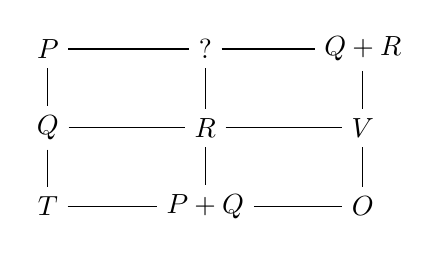
\begin{tikzpicture}
\node(t) at (0, 0) {$ T $};
\node(pq) at (2, 0) {$ P + Q $};
\node(o) at (4, 0) {$ O $};
\node(q) at (0, 1) {$ Q $};
\node(r) at (2, 1) {$ R $};
\node(v) at (4, 1) {$ V $};
\node(p) at (0, 2) {$ P $};
\node(pqr) at (2, 2) {$ ? $};
\node(qr) at (4, 2) {$ Q + R $};
\draw (p) -- (pqr) -- (qr);
\draw (q) -- (r) -- (v);
\draw (t) -- (pq) -- (o);
\draw (p) -- (q) -- (t);
\draw (pqr) -- (r) -- (pq);
\draw (qr) -- (v) -- (o);
\end{tikzpicture}
\end{center}

Need to show that $ ? $ lies on the cubic, that is if we find the unique point of intersection of the line joining $ P + Q $ and $ R $, with the line joining $ P $ and $ Q + R $, this lies on the cubic we are considering. Apply Lemma \ref{lem:5.7} to the eight points $ O, P, Q, R, T, V, P + Q, Q + R $. Consider the cubic given by the union of the three horizontal lines, and the cubic given by the union of the three vertical lines. So the ninth point in Lemma \ref{lem:5.7} is $ ? $. Since the eight points all lie on our cubic, Lemma \ref{lem:5.7} gives $ ? $ lies on the cubic, as required.

\begin{definition}
An \textbf{elliptic curve} over a field $ k $ is a nonsingular plane cubic $ E $ together with a fixed choice of $ O $ defined over $ k $.
\end{definition}

\begin{definition}
A \textbf{point of inflexion} on a nonsingular plane cubic is a point where the tangent line does not meet the curve again, that is it meets the curve with multiplicity three.
\end{definition}

\begin{lemma}
\label{lem:5.10}
If $ E $ is an elliptic curve and $ O $ is chosen to be a point of inflexion, then $ P + Q + R = O $ iff $ P, Q, R $ are collinear.
\end{lemma}

\begin{proof}
TODO Exercise.
\end{proof}

\begin{lemma}
Consider the cubic $ y^2 = f\rb{x} $, where $ f\rb{x} $ is monic of degree three.
\begin{enumerate}
\item This curve has a unique point at infinity, which is nonsingular.
\item The point at infinity is a point of inflexion.
\item The cubic is irreducible, and if $ char\rb{k} \ne 2 $, then the cubic is nonsingular iff $ f\rb{x} $ has distinct roots.
\end{enumerate}
\end{lemma}

\begin{proof}
\hfill
\begin{enumerate}
\item $ Y^2Z - X^3 - aX^2Z - bXZ^2 - cZ^3 $. Points at infinity have $ Z = 0 $, so $ X^3 = 0 $, so $ \sb{0 : 1 : 0} $ is the only point at infinity. $ \partial / \partial Z = Y^2 \ne 0 $ at $ \sb{0 : 1 : 0} $.
\item Since $ \partial / \partial X = \partial / \partial Y = 0 $ at $ \sb{0 : 1 : 0} $, the tangent line through $ \sb{0 : 1 : 0} $ is just $ Z = 0 $. So the tangent line meets the curve at points where $ Z = 0 $, that is at $ \sb{0 : 1 : 0} $.
\item (TODO Exercise: irreducibility) Nonsingular points at infinity. For $ y^2 - f\rb{x} $, $ \partial / \partial y = 2y $, so any singular point would have $ y = 0 $ using $ char\rb{k} \ne 2 $. $ \partial / \partial x = -f'\rb{x} $, so a singular point would need $ f\rb{x} = f'\rb{x} = 0 $, that is you need a repeated root of $ f $.
\end{enumerate}
\end{proof}

A fact is that any nonsingular plane cubic with a given point $ O $ can be put into the form $ y^2 + \gamma xy + \delta y = g\rb{x} $, with $ g\rb{x} $ a cubic, and the given point $ O $ being sent to infinity, by the Riemann-Roch theorem. If $ char\rb{k} \ne 2 $, can complete the square to get rid of the $ xy, y $ terms. If $ char\rb{k} \ne 3 $, can complete the cube, so we can assume that the elliptic curve is $ y^2 = x^3 + ax + b $. Lines through $ O = \sb{0 : 1 : 0} $ are lines $ x = k $ for some $ k $. If $ T = \rb{x_0, y_0} $, then $ P + Q = \rb{x_0, -y_0} $. In fact, since $ O $ is a point of inflexion, we can compute $ P $ as follows. Since $ P + \rb{-P} = O $ so $ O + P + \rb{-P} = O $, so by Lemma \ref{lem:5.10}, $ O, P, -P $ are collinear. So if $ P = \rb{x_1, y_1} $ then $ -P = \rb{x_1, -y_1} $. In particular, $ 2P = O $ iff $ P = O $ or $ P = \rb{x, 0} $ for some $ x $, that is the points with $ 2P = O $ are $ O $ and $ \rb{\alpha, 0}, \rb{\beta, 0}, \rb{\gamma, 0} $ where $ \alpha, \beta, \gamma $ are the roots of $ X^3 + aX + b $. The discriminant $ \Delta $ of $ y^2 = x^3 + ax + b $ is by definition the discriminant of $ x^3 + ax + b $, which is $ 4a^3 + 27b^2 $. So this is an elliptic curve iff $ x^3 + ax + b $ has three distinct roots, iff $ 4a^3 + 27b^2 \ne 0 $.

\marginpar{Lecture 18 \\ Tuesday \\ 13/11/18}

(TODO Exercise: the only changes of variable that take the equation $ y^2 = x^3 + ax + b $ to an equation of the same form are those of the form $ x' = u^2x $ and $ y' = u^3y $. Such a change of variables scales $ a $ by $ u^4 $ and $ b $ by $ u^6 $, so $ \Delta $ changes by $ u^{12} $.)

\begin{definition}
Let $ E $ be the elliptic curve $ y^2 = x^3 + ax + b $. Then $ j\rb{E} = -1728\rb{4a}^3 / \Delta $. This is called the \textbf{$ j $-invariant} of $ E $.
\end{definition}

\begin{proposition}
If $ k $ is algebraically closed, then two elliptic curves $ E $ and $ E' $ are isomorphic iff $ j\rb{E} = j\rb{E'} $.
\end{proposition}

\begin{proof}
Assume $ char\rb{k} \ne 2, 3 $, so that $ y^2 = x^3 + ax + b $ is $ E $ and $ y^2 = x^3 + Ax + B $ is $ E' $. If the two curves are isomorphic, then we can find $ u $ such that $ A = u^4a $ and $ B = u^6B $ and then $ j\rb{E} = j\rb{E'} $. Suppose conversely that $ j\rb{E} = j\rb{E'} $, that is $ A^3 / \rb{4A^3 + 27B^2} = a^3 / \rb{4a^3 + 27b^2} $, that is $ B^2 / A^3 = b^2 / a^3 $, that is $ \rb{B / b}^2 = \rb{A / a}^3 $, assuming that $ a, b, A, B \ne 0 $. Choose $ u $ such that $ u^{12} = \rb{B / b}^2 = \rb{A / a}^3 $. Modifying $ u $ by an appropriate twelfth root of unity, we can arrange that $ A / a = u^4 $, $ B / b = u^6 $. Then $ y' = u^3y $, $ x' = u^2x $ gives the required change of variables. It remains to consider the cases that some of $ a, b, A, B $ are zero. Writing the equation as $ A^3b^2 = a^3B^2 $, if $ A = 0 $ then $ B \ne 0 $ as $ 4A^3 + 27B^2 \ne 0 $, so $ a^3 = 0 $ and $ a = 0 $. Similarly $ B = 0 $ iff $ b = 0 $. In the first case $ A = a = 0 $, choose $ u $ such that $ B / b = u^6 $. In the second case $ B = b = 0 $, choose $ u $ such that $ A / a = u^4 $.
\end{proof}

Return to the case of irreducible singular cubics. Write as $ y^2 = f\rb{x} $, $ f\rb{x} $ a monic cubic, then this is singular iff $ f\rb{x} $ has a repeated root. There are two cases.
\begin{enumerate}
\item All three roots are equal, so $ y^2 = x^3 $. The only singular point is $ \rb{0, 0} $. Consider the group law with $ 0 = \sb{0 : 1 : 0} $. Because $ \sb{0 : 1 : 0} $ is a point of inflexion, Lemma \ref{lem:5.10} tells us that three points add to $ O $ iff they are collinear. Consider a line of the form $ ax + by = 1 $. This is the general form of a line not going through $ \rb{0, 0} $. $ x^3 = y^2 = y^2\rb{1} = y^2\rb{ax + by} $. Since $ \rb{x, y} \ne 0 $ we actually have $ y \ne 0 $, so we can divide by $ y $ and get $ \rb{x / y}^3 = a\rb{x / y} + b $. This is a cubic in $ x / y $, with no quadratic term. Conversely, any cubic in $ x / y $ with no quadratic term is of this form for some $ a, b $. So we see that $ \rb{x_1, y_1} + \rb{x_2, y_3} + \rb{x_3, y_3} = O $ iff $ x_1 / y_1 + x_2 / y_2 + x_3 / y_3 = 0 $. So in this case by mapping $ \rb{x, y} \mapsto x / y $ we get that the group law is given by the usual additive group.
\item Two roots are equal and the third is distinct, so $ y^2 = x^2\rb{x + 1} $. Again $ \rb{0, 0} $ is singular. $ x^3 = y^2 - x^2 = \rb{y + x}\rb{y - x} $. Let $ U = y + x $ and $ V = y - x $, so $ \rb{U - V}^3 = 8UV $. Again $ \rb{0, 0} $ is the only singular point. Consider lines $ aU + bV = 1 $. $ \rb{U - V}^3 = 8UV\rb{1} = 8UV\rb{aU + bV} $. Write $ t = U / V $, get $ \rb{t - 1}^3 = 8t\rb{at + b} $, so $ t^3 - \rb{8a + 3}t^2 + \rb{8b + 3}t - 1 = 0 $. So we have a general monic cubic with constant term $ -1 $, that is with roots having product equal to one. So sending $ \rb{x, y} \mapsto U / V = \rb{y + x} / \rb{y - x} $ gives an isomorphism between the group law on $ y^2 = x^2\rb{x + 1} $ and the group $ k^* $ under multiplication.
\end{enumerate}

\marginpar{Lecture 19 \\ Thursday \\ 15/11/18}

Doubling and addition formulae in $ y^2 = x^3 + ax + b $ for $ P = \rb{x_1, y_1} $ and $ Q = \rb{x_2, y_2} $ are
$$ P + Q = \dfrac{-2y_1y_2 + \rb{x_1 + x_2}\rb{x_1x_2 + a} + 2b}{\rb{x_1 - x_2}^2}, $$
$$ 2P = \dfrac{x_1^4 - 2ax_1^2 - 8bx_1 + a^2}{4\rb{x_0^3 + ax_0 + b}}. $$

\begin{example}
Good way to practice explicit computations is to work over small fields. Let $ k = \F_5 = \Z / 5\Z $ be the field of five elements and $ y^2 = x^3 + 1 $. $ \Delta = 4 \ne 0 $ in $ k $. So this is an elliptic curve. Squares modulo five are $ 0, 1, 4 $.
\begin{center}
\begin{tabular}{c|ccccc}
$ x $ & $ 0 $ & $ 1 $ & $ 2 $ & $ 3 $ & $ 4 $ \\
\hline
$ y $ & $ \pm 1 $ & & $ \pm 2 $ & & 0
\end{tabular}
\end{center}
Also $ O = \sb{0 : 1 : 0} $. So six points in total. Since $ \Z / 6\Z \cong \Z / \Z / 2\Z \times \Z / 3\Z $ by the Chinese remainder theorem, the points form an abelian group of order six. $ \rb{4, 0} $ is the only point of order two. The line $ Y = Z $ meets the curve at $ \rb{0, 1} $ in projective coordinates, and is actually the tangent line at this point, so this point has order three. If we are identifying our group of points with $ \Z / 6\Z $, then we have to identify $ \rb{4, 0} $ with $ 3 + 6\Z $, $ \rb{0, 1} $ with $ \pm 2 + 6\Z $, and $ \rb{0, -1} = -\rb{0, 1} $ with $ \mp 2 + 6\Z $. So $ \rb{2, \pm 2} $ must be the points of order six. More explicitly, the line through $ \rb{4, 0} $ and $ \rb{0, 1} $ is $ y = x + 1 $, which also passes through $ \rb{2, -2} $. So $ \rb{4, 0} + \rb{0, 1} + \rb{2, -2} = O $, so $ \rb{4, 0} + \rb{0, 1} = -\rb{2, -2} = \rb{2, 2} $. (TODO Exercise: figure out $ n\rb{2, 2} $ for $ 1 \le n \le 5 $)
\end{example}

For $ E $ an elliptic curve, $ E\rb{k} $ are the points of $ E $ with coordinates in $ k $, including $ O = \sb{0 : 1 : 0} $. If $ k \subset K $, $ E\rb{K} $ are the points with coordinates in $ K $.

\begin{example}
If $ k $ is a finite field, then $ E\rb{k} $ is either cyclic or a product of two cyclic groups, by the Hasse bound or Hasse-Weil bound on number of points.
\end{example}

\begin{example}
If $ k = \C $, $ E\rb{\C} \cong \C / \Lambda $ as abelian groups or Riemann surfaces, where $ \Lambda \subset \C $ is a lattice, that is a subgroup isomorphic to $ \Z^2 $. Over $ \C $, we have exactly $ n^2 $ points $ P $ with the property that $ nP = O $. These points are just
$$ \dfrac{\tfrac{1}{n}\Lambda}{\Lambda} \cong \dfrac{\tfrac{1}{n}\Z^2}{\Z^2} \cong \dfrac{\Z^2}{n\Z^2} \cong \rb{\dfrac{\Z}{n\Z}}^2. $$
\end{example}

\begin{definition}
We say that $ P $ is an \textbf{$ n $-torsion point} if $ nP = O $. Say that $ P $ is \textbf{torsion} if it is $ n $-torsion for some $ n \ge 1 $. The set of $ n $-torsion points is a group, because if $ nP = O $, $ nQ = O $, then $ n\rb{-P} = -\rb{nP} = -O = O $, and $ n\rb{P + Q} = nP + nQ = O + O = O $. Write $ E\rb{k}\sb{n} $ for the $ n $-torsion points of $ E\rb{k} $.
\end{definition}

\begin{example}
We just saw that $ E\rb{C}\sb{n} \cong \rb{\Z / n\Z}^2 $.
\end{example}

$ k = \Q_p $ is the next few lectures. $ E\rb{\Q_p} $ is locally isomorphic to $ \Z_p $. Approximation of formal groups in the next few lectures. $ k = \Q $ is the Mordell-Weil theorem. $ E\rb{\Q} $ is a finitely generated abelian group, that is there is a surjection $ \Z^N \twoheadrightarrow E\rb{\Q} $ for some $ N $. Structure theorem for finitely generated abelian groups states that any finitely generated abelian group is isomorphic to a group of the form $ \Z^r \oplus X $, where $ X $ is finite. Furthermore, $ r $ is uniquely determined, as is the isomorphism classes of $ X $. Call $ r $ the \textbf{rank} of the group. In fact if $ G $ is a finitely generated abelian group. We can write $ G \cong G^{free} \times G_{tor} $, where $ G^{free} \cong \Z^r $ for some $ r $, and $ G_{tor} $ are the elements of $ G $ of finite order, which are the elements which are $ n $-torsion for some $ n $. $ G_{tor} $ is a finite group.

\end{document}
